\chapter{Технологическая часть}

\section{Средства реализации}

\subsection*{Язык программирования}

Для реализации ПО был выбран язык программирования C++~\cite{cpp} стандарта ``C++20'' по следующим причинам:
\begin{itemize}
  \item данный язык является объектно-ориентированным, что позволяет проектировать сложные системы взаимодействия объектов для обработки и визуализации;
  \item стандартная библиотека языка достаточна для осуществления всех спроектированных алгоритмов;
  \item стандартная библиотека языка предоставляет средства для профилирования и исследования временных затрат;
  \item для языка разработано большое количество библиотек, расширяющих возможности языка. 
\end{itemize}

В процессе разработки ПО были использованы внешние библиотеки:
\begin{itemize}
  \item Qt6~\cite{qt} для осуществления интерфейса программы;
  \item OneApi TBB~\cite{tbb} для параллелизации процессов.
\end{itemize}

\subsection*{Система сборки}

В качестве системы сборки проекта была выбрана система CMake~\cite{CMake}, так как она предназначена для работы с языками C и C++ и предоставляет возможность контроля над подключаемыми файлами и библиотеками.

\subsection*{Среда разработки}

Для разработки была выбрана Visual Studio Code~\cite{vscode}, так как она предоставляет достаточный интерфейс для написания и отладки кода, а также обеспечивает возможность работы с избранной системой сборки.

Для редактирования интерфейса была использована программа QtDesigner, поставляемая вместе с библиотекой Qt.

\section{Структура классов}

Были разработаны следующие классы:
\begin{itemize}
  \item \emph{Point2D} --- для работы с точками на плоскости;
  \item \emph{Point3D} --- для работы с точками в пространстве;
  \item \emph{Triangle} --- для работы с треугольниками в пространстве;
  \item \emph{Plane} --- для работы с плоскостями;
  \item \emph{Color} --- описывающий цвет;
  \item \emph{Face} --- для работы с гранями объектов;
  \item \emph{Square} --- класс, описывающий квадрат в пространстве;
  \item \emph{Cube} --- класс, описывающий куб в пространстве;
  \item \emph{BaseModel} --- базовый класс модели на сцене;
  \item \emph{FaceModel} --- класс для работы с поверхностными моделями;
  \item \emph{House} --- класс, описывающий модель дома;
  \item \emph{Tree} --- класс, описывающий модель дерева;
  \item \emph{RoadXX} --- классы, описывающие модели дорог разных видов;
  \item \emph{TransformationMatrix} --- класс, описывающий матрицу трансформации моделей;
  \item \emph{Scene} --- класс, хранящий объекты сцены;
  \item \emph{BaseCamera} --- базовый класс, описывающий камеры;
  \item \emph{PerspectiveCamera} --- камера, отображающая точки по принципу перспективной проекции;
  \item \emph{ShadowMap} --- класс, предоставляющий доступ к карте теней;
  \item \emph{BaseVisitor} --- базовый класс для паттерна программирования ``посетитель'';
  \item \emph{ShadowMapVisitor} --- ``посетитель'', производящий вычисление карты теней;
  \item \emph{RenderVisitor} --- ``посетитель'', производящий вычисление буфера кадра;
  \item \emph{QWFC} --- класс, осуществляющий генерацию матрицы сцены;
  \item \emph{Cell} --- класс, описывающий ячейку для алгоритма QWFC;
  \item \emph{Rule} --- класс, описывающий правило для алгоритма QWFC.
\end{itemize}

Схема разработанных классов изображена на рисунке~\ref{fig:UML}.

\begin{figure}[h]
  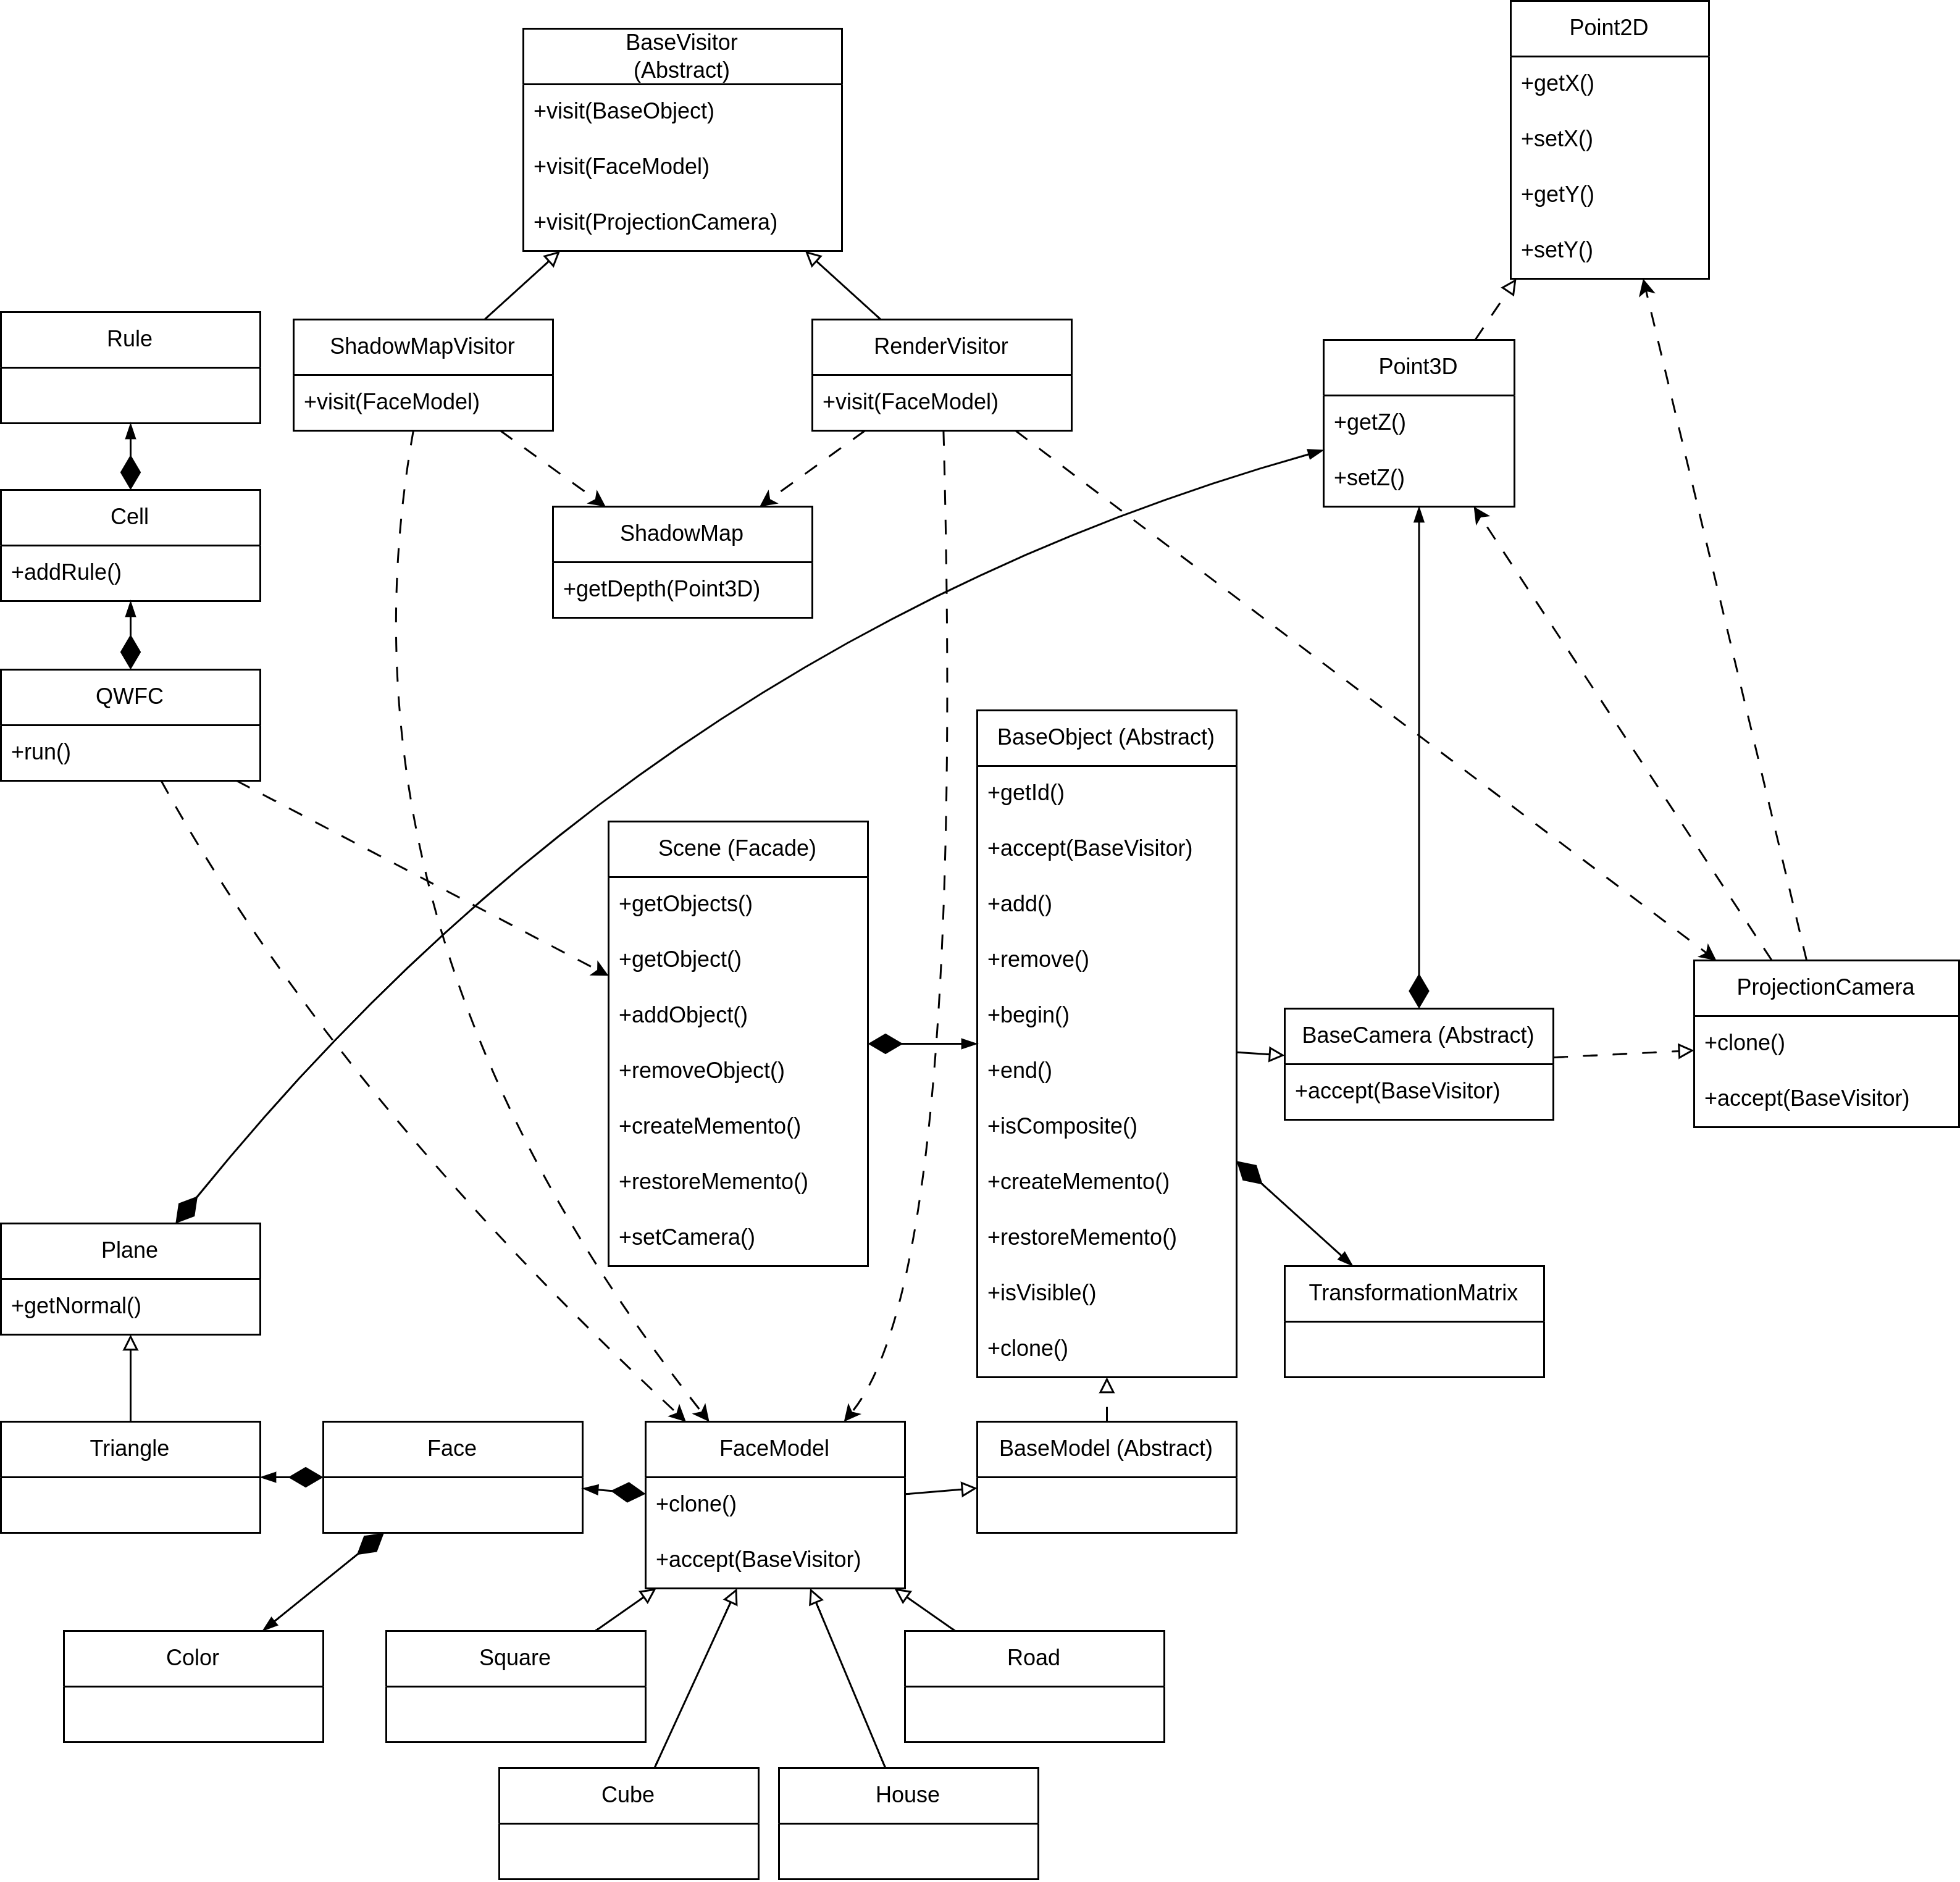
\includegraphics[width=\textwidth]{diagram.drawio.png}
  \caption{Диаграмма классов}
  \label{fig:UML}
\end{figure}

Из перечисления выше исключены те классы и структуры, которые используются только для связи с интерфейсом и библиотекой Qt во избежание загромождения.

\section{Реализация ПО}

Процесс отрисовки изображения с помощью алгоритма Z-буфера происходит при использовании класса RenderVisitor на сцену. 
Эта функция представлена на листинге~\ref{lst:render_scene}. 

На этом этапе происходит инициализация буфера глубины и кадра. Затем RenderVisitor обрабатывает каждый объект на сцене. Этот процесс происходит с использованием библиотеки tbb, поэтому каждый объект обрабатывается параллельно, что позволяет сильно сократить время создания кадра (см. исследовательскую часть).

Поскольку алгоритм Z-буфера не рассчитан на одновременную обработку несколькими потоками, каждый объект создаёт набор буферов кадра, которые затем объединяются для получения выходного изображения.

Функция обработки модели объектом RenderVisitor представлена на листинге~\ref{lst:render_model}.

Из каждого объекта извлекаются грани, затем происходит фильтрация алгоритмами отсечения невидимых поверхностей невидимых граней. Оставшиеся грани создают буферы кадра и сохраняют их в общий массив. Обработка каждой грани также происходит одновременно. Поскольку все грани представляются треугольниками, процесс растеризации был оптимизирован для них. 
Координаты глубины и мировых координат вычисляются итерационно для каждой сканирующей строки треугольника в соответствии с алгоритмом, разработанным в аналитической части.
Также в этом методе происходит сравнение координат точек с координатами в карте теней.

Вычисление карты теней выполняется аналогично заполнению глубины буфера кадра, но вместо матрицы преобразования камеры используется матрица преобразования источника света.

Заполнение буфера кадра сцены происходит когда изменяется сцена, то есть меняется положение и/или направление камеры, изменяется положение источника света или изменяются объекты на сцене.

Расчёт карты теней происходит только при изменении положения источника света или изменении объектов на сцене.

Метод collapseCell класса QWFC представлен на листинге~\ref{lst:qwfcoll}. Фиксирование состояния ячейки производится в соответствии с приоритетами, их учёт можно увидеть в этой функции.

После фиксирования состояния ячейки состояние соседних ячеек рекурсивно обновляется.

Для тестирования алгоритма QWFC, вместе с основным файлом программы ``app'', собирается файл ``qwf'', производящий замеры времени генерации сцены.

\section*{Пользовательский интерфейс}

Пользовательский интерфейс состоит из описанных ниже групп управления.

\subsection*{Группа управления генерацией сцены}

В данной группе управления пользователю доступны:
\begin{itemize}
  \item два поля ввода для задания размеров матрицы сцены;
  \item четыре поля ввода для задания вероятностей появления разных типов объектов;
  \item кнопка ``создать'', осуществляющая генерацию новой сцены.
\end{itemize}

\subsection*{Группа управления положения источника света}

В данной группе управления пользователю доступны два ползунка для управления поворотом источника вокруг осей $Ox$ и $Oy$.

Управление камерой производится с помощью клавиатуры:
\begin{itemize}
  \item клавиши ``W'', ``A'', ``S'', ``D'' используются для движения камеры вперёд, влево, назад и вправо соответственно;
  \item клавиши ``I'', ``J'', ``K'', ``L'' используются для поворотов камеры вверх, влево, вниз и вправо соответственно;
  \item клавиши ``Пробел'' и ``B'' используются для движения камеры вверх и вниз вдоль оси $Oy$ соответственно.
\end{itemize}



\section{Демонстрация работы программы}

На рисунках~\ref{fig:example_1}-\ref{fig:example_5} представлены примеры работы программы.

\begin{figure}[h!]
  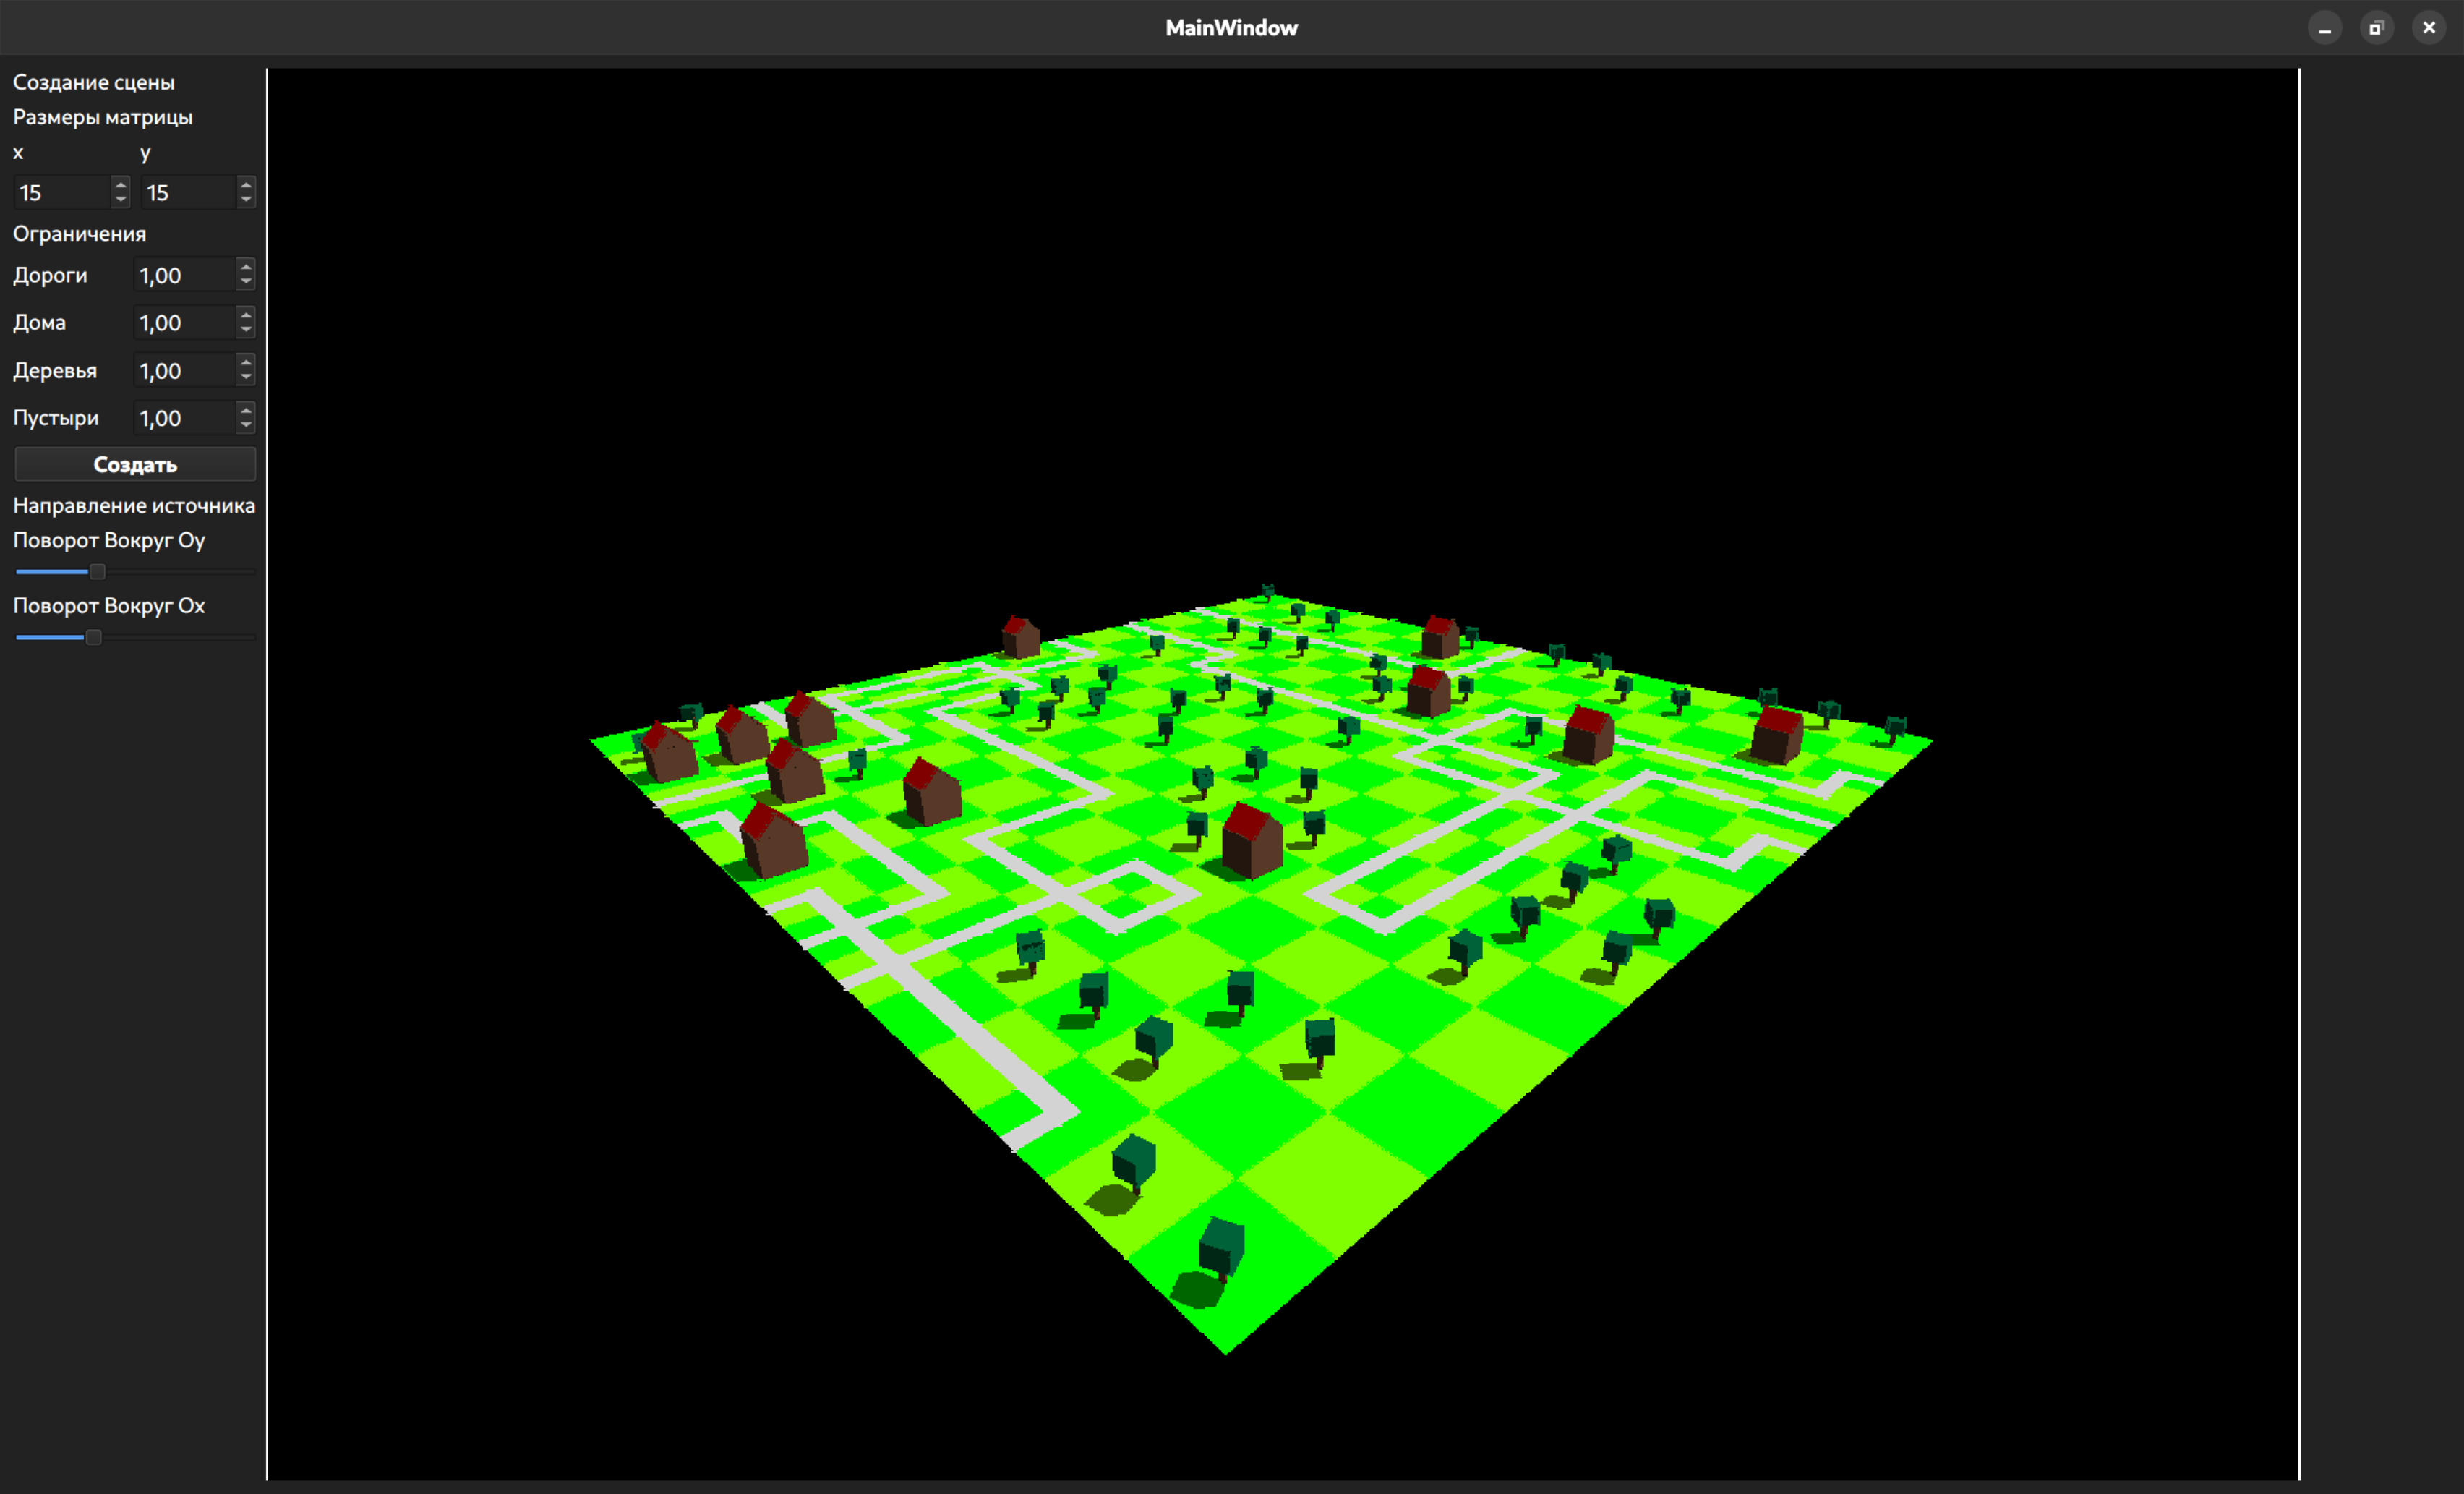
\includegraphics[width=\textwidth]{pic1}
  \caption{Пример работы программы --- генерация посёлка 15 на 15 ячеек}
  \label{fig:example_1}
\end{figure}
\begin{figure}[h!]
  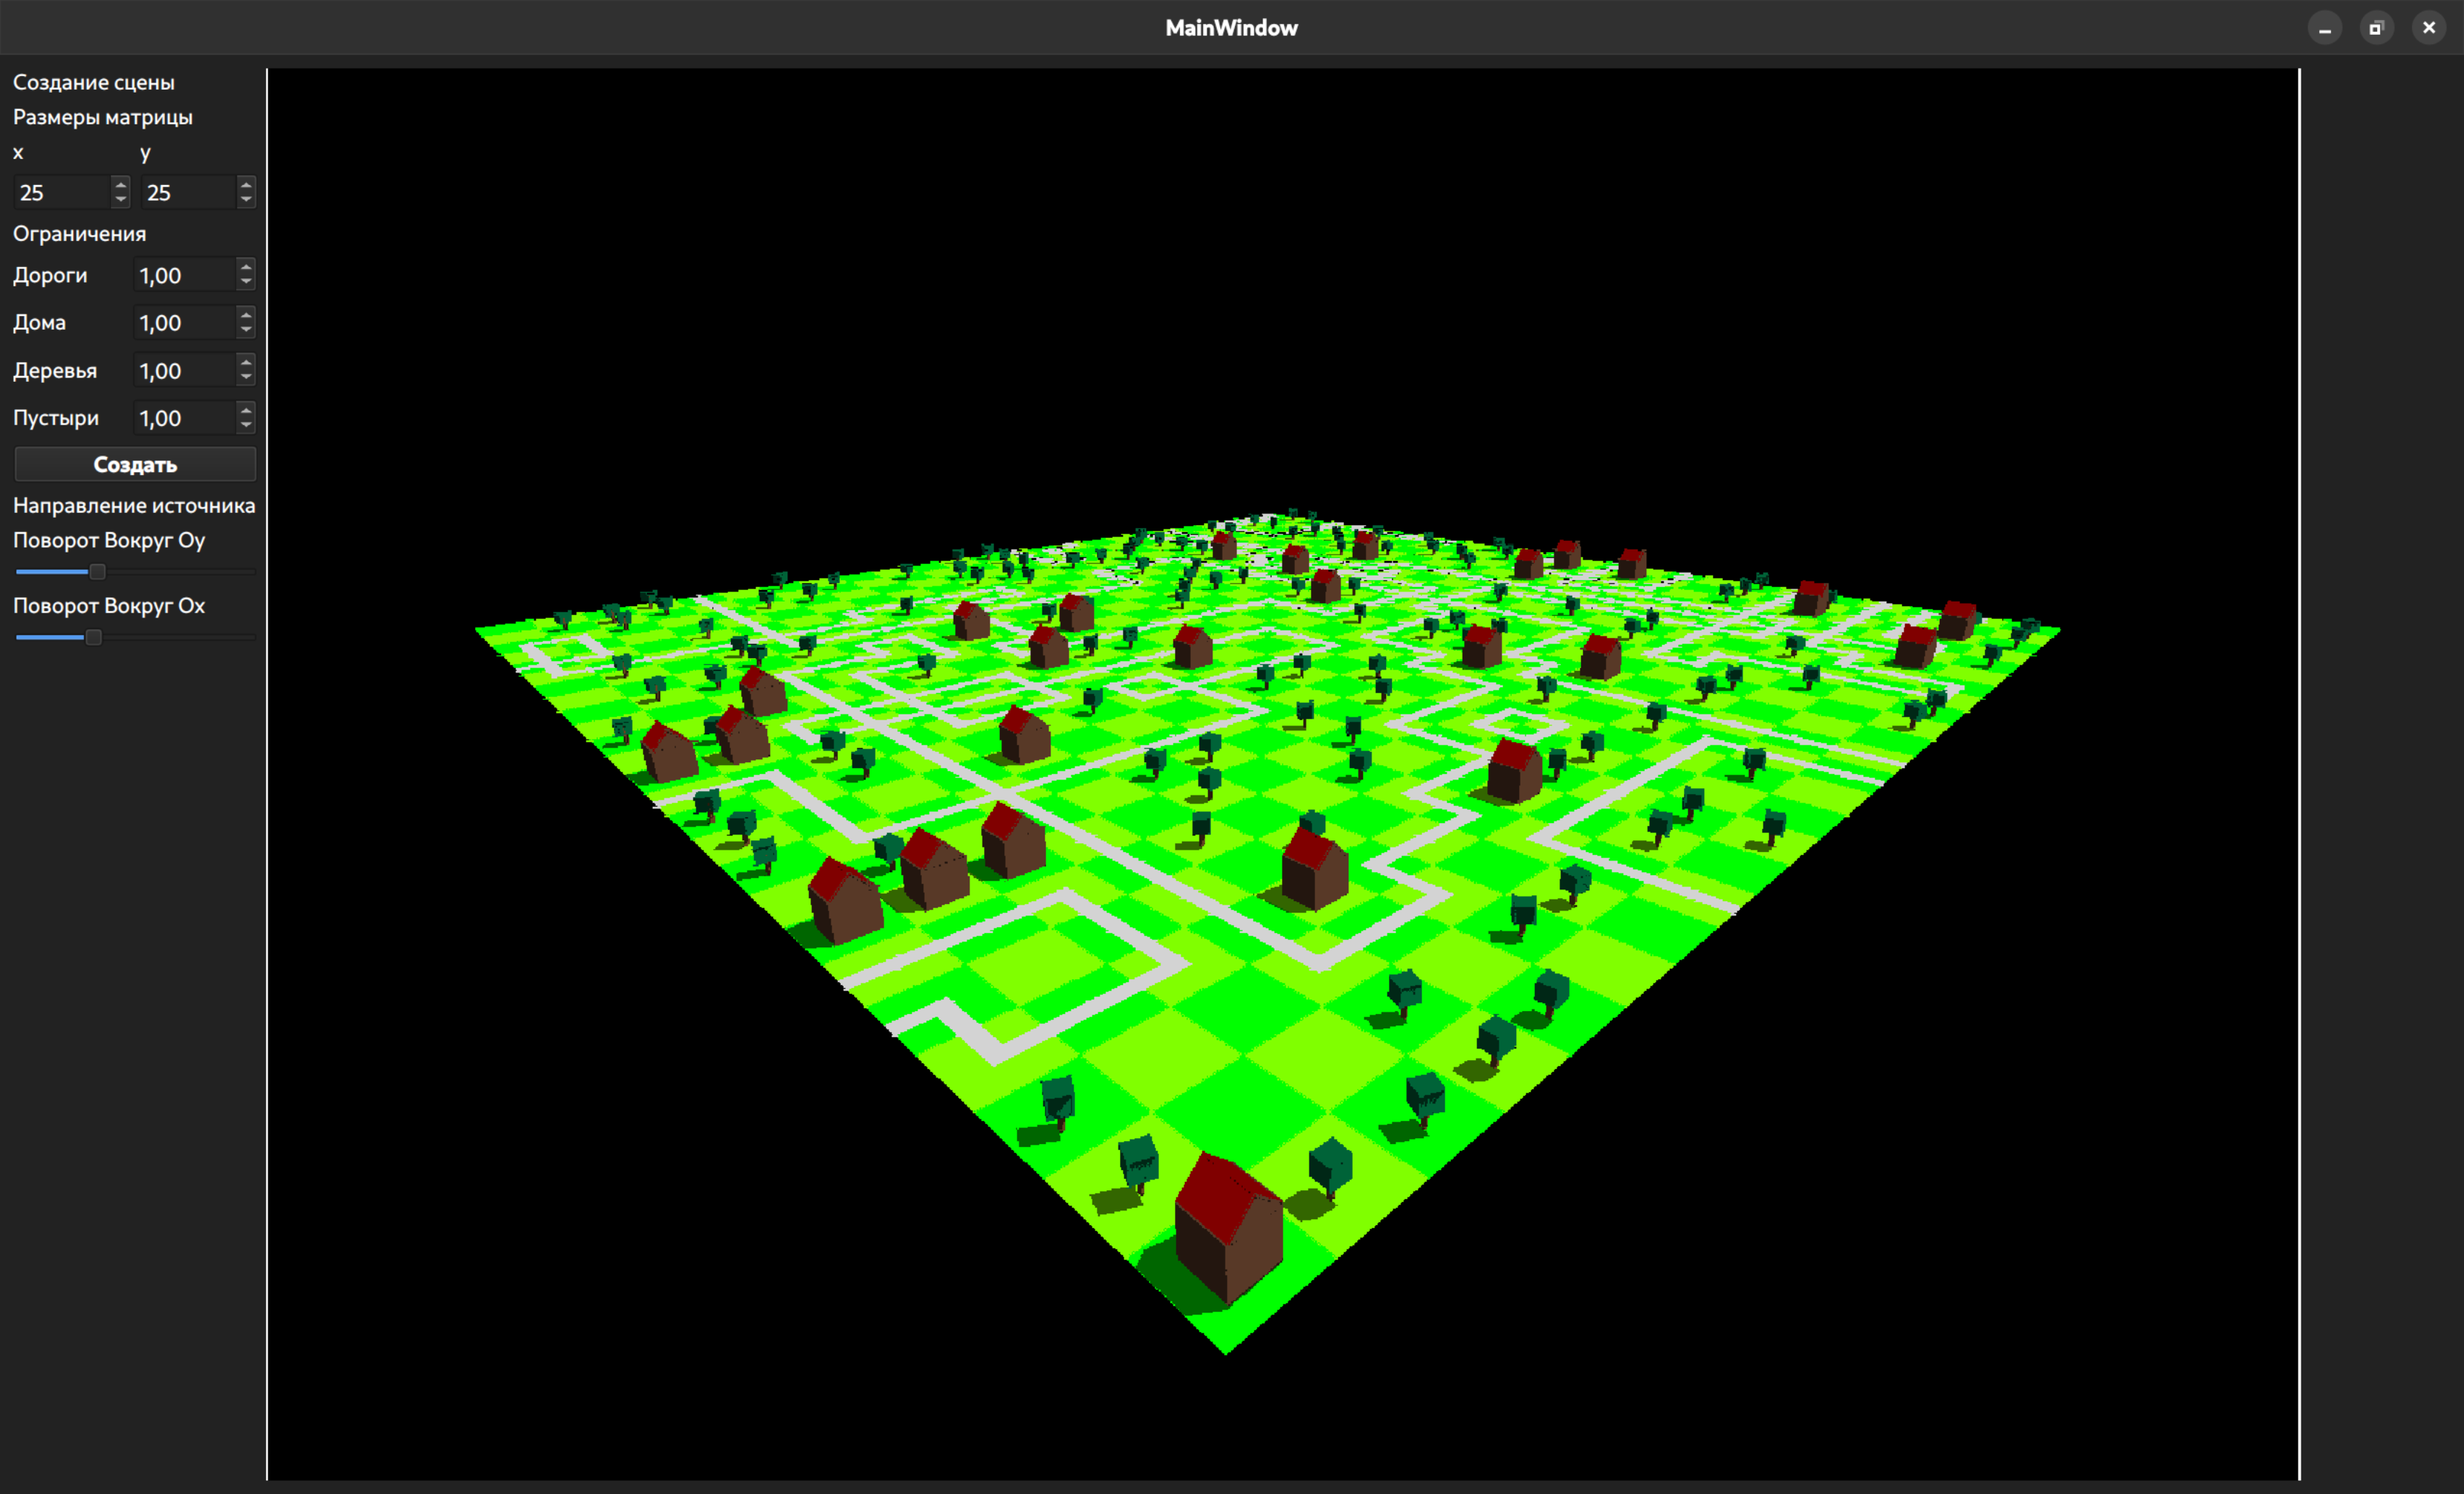
\includegraphics[width=\textwidth]{pic2}
  \caption{Пример работы программы ---  генерация посёлка 25 на 25 ячеек}
  \label{fig:example_2}
\end{figure}
\begin{figure}[h!]
  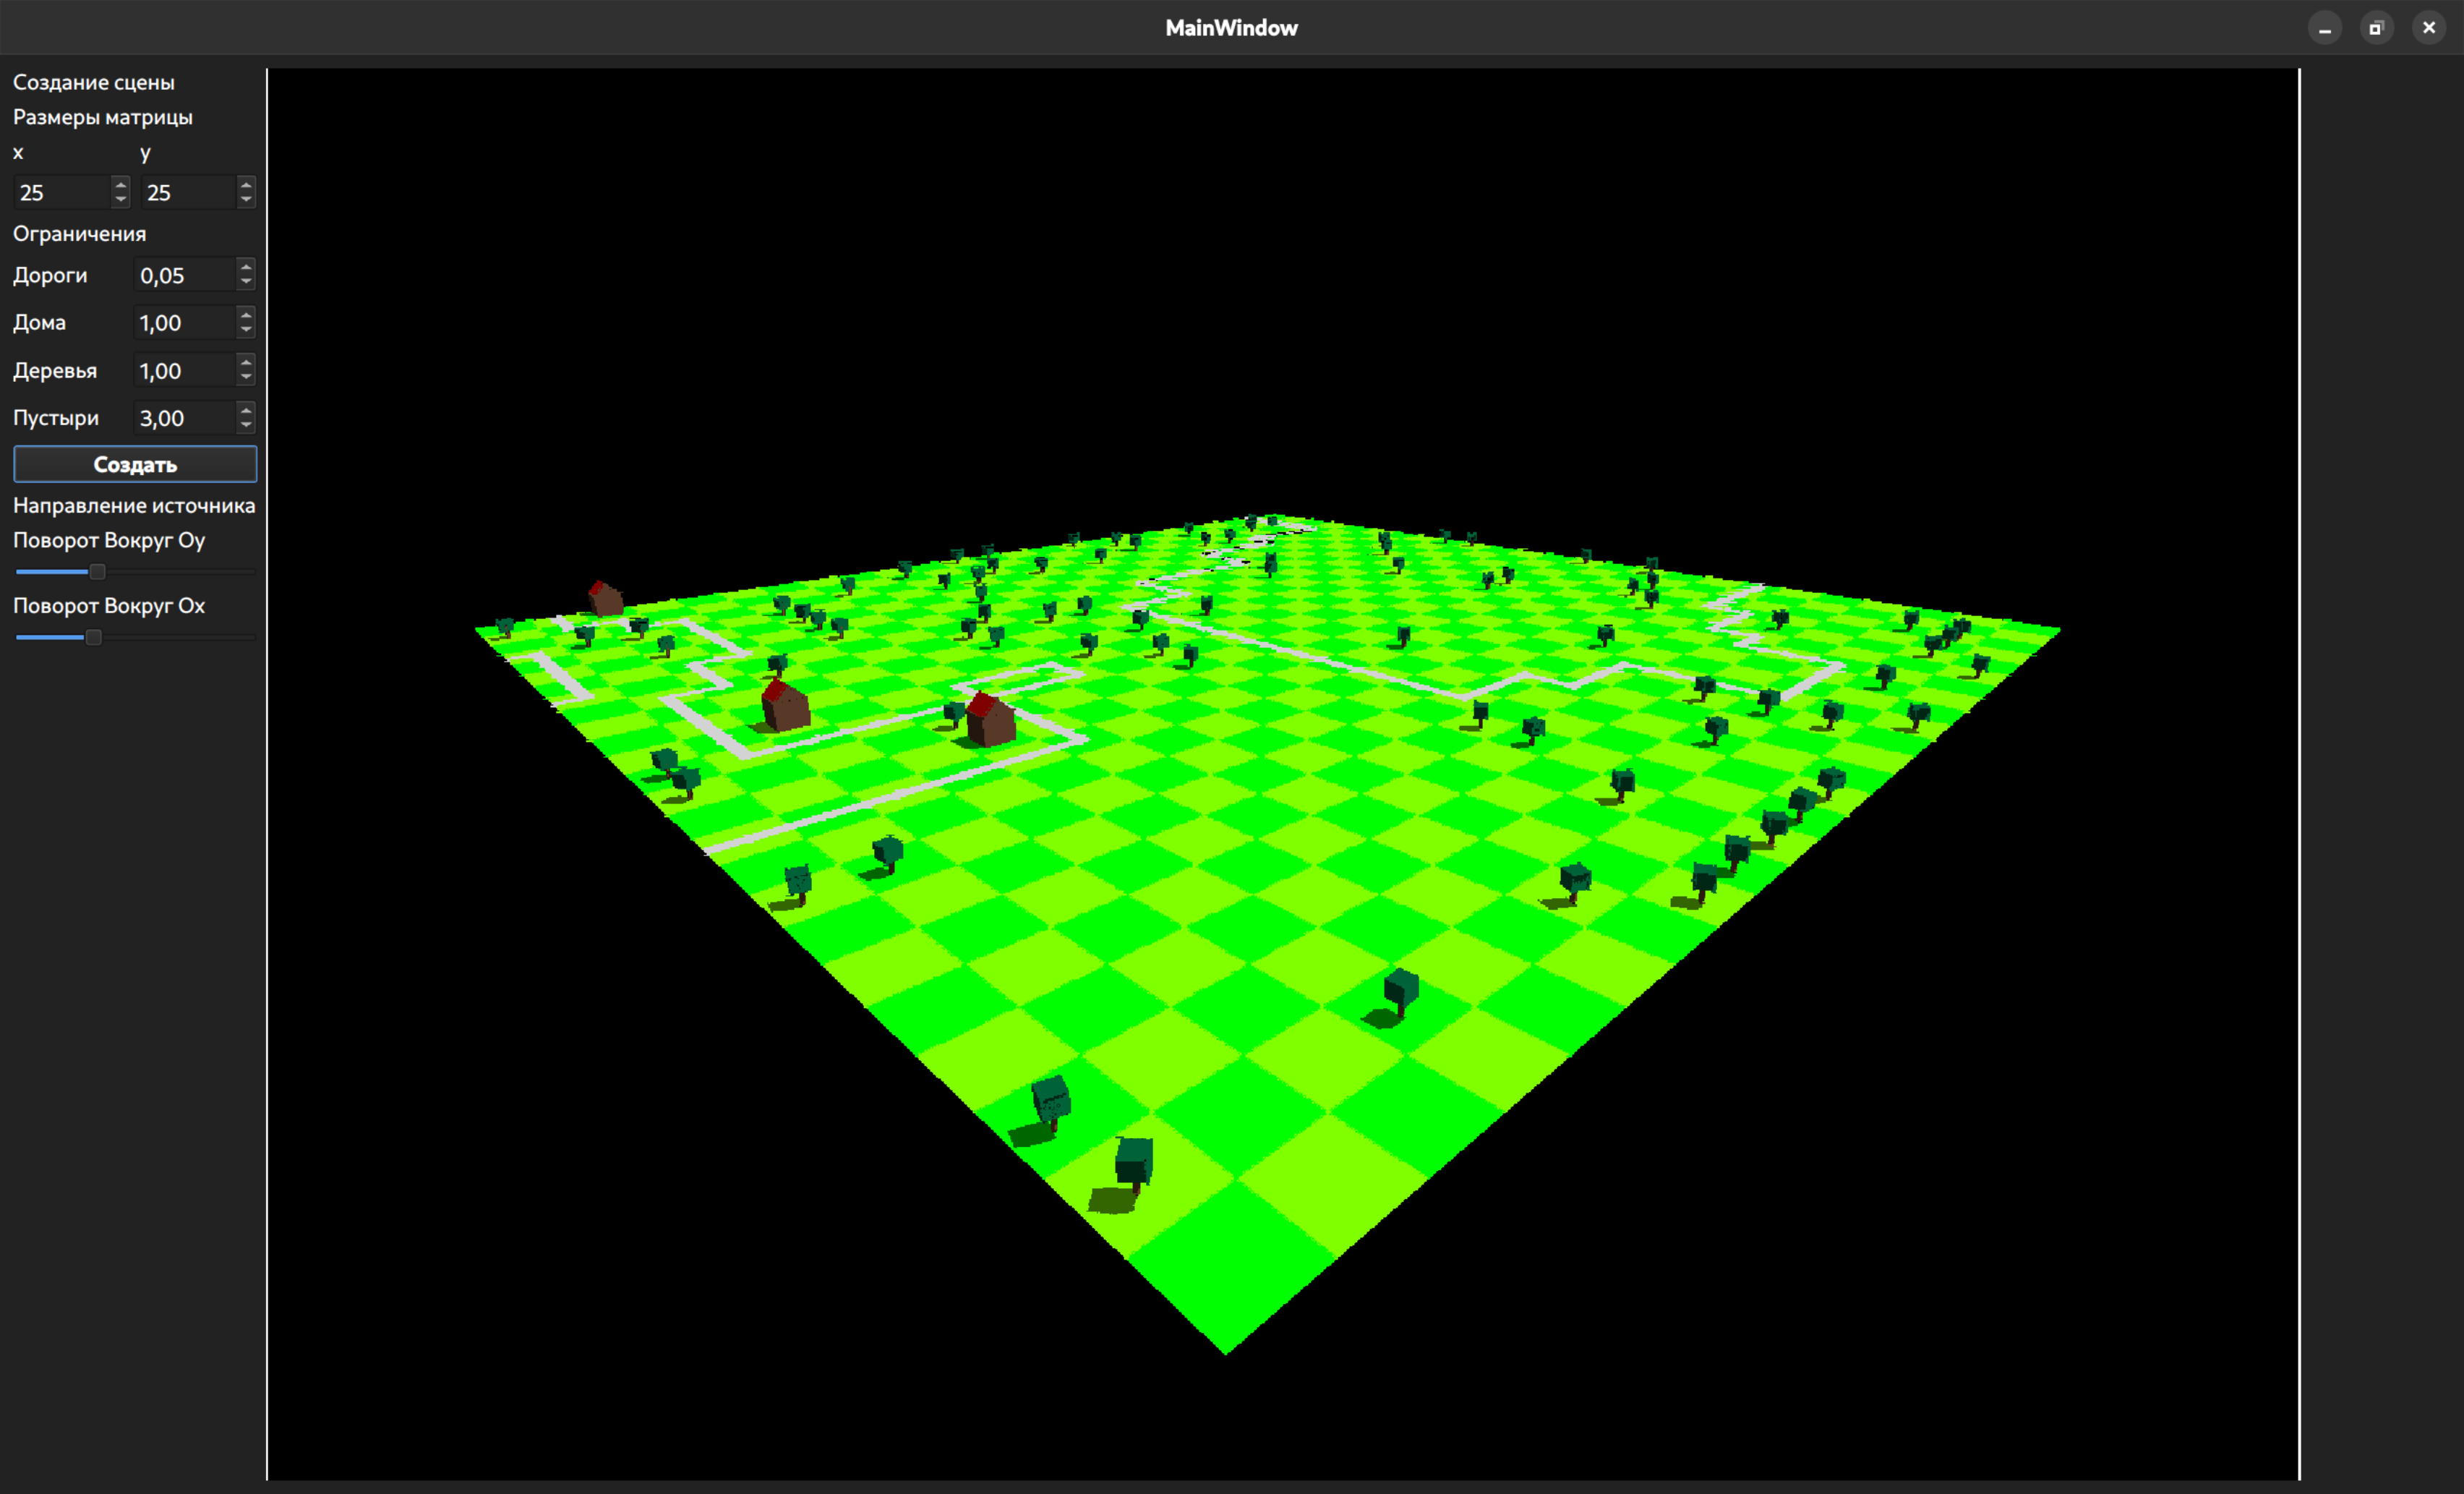
\includegraphics[width=\textwidth]{pic3}
  \caption{Пример работы программы --- генерация посёлка с уменьшенным количеством дорог и увеличенным колчичеством пустырей}
  \label{fig:example_3}
\end{figure}
\begin{figure}[h!]
  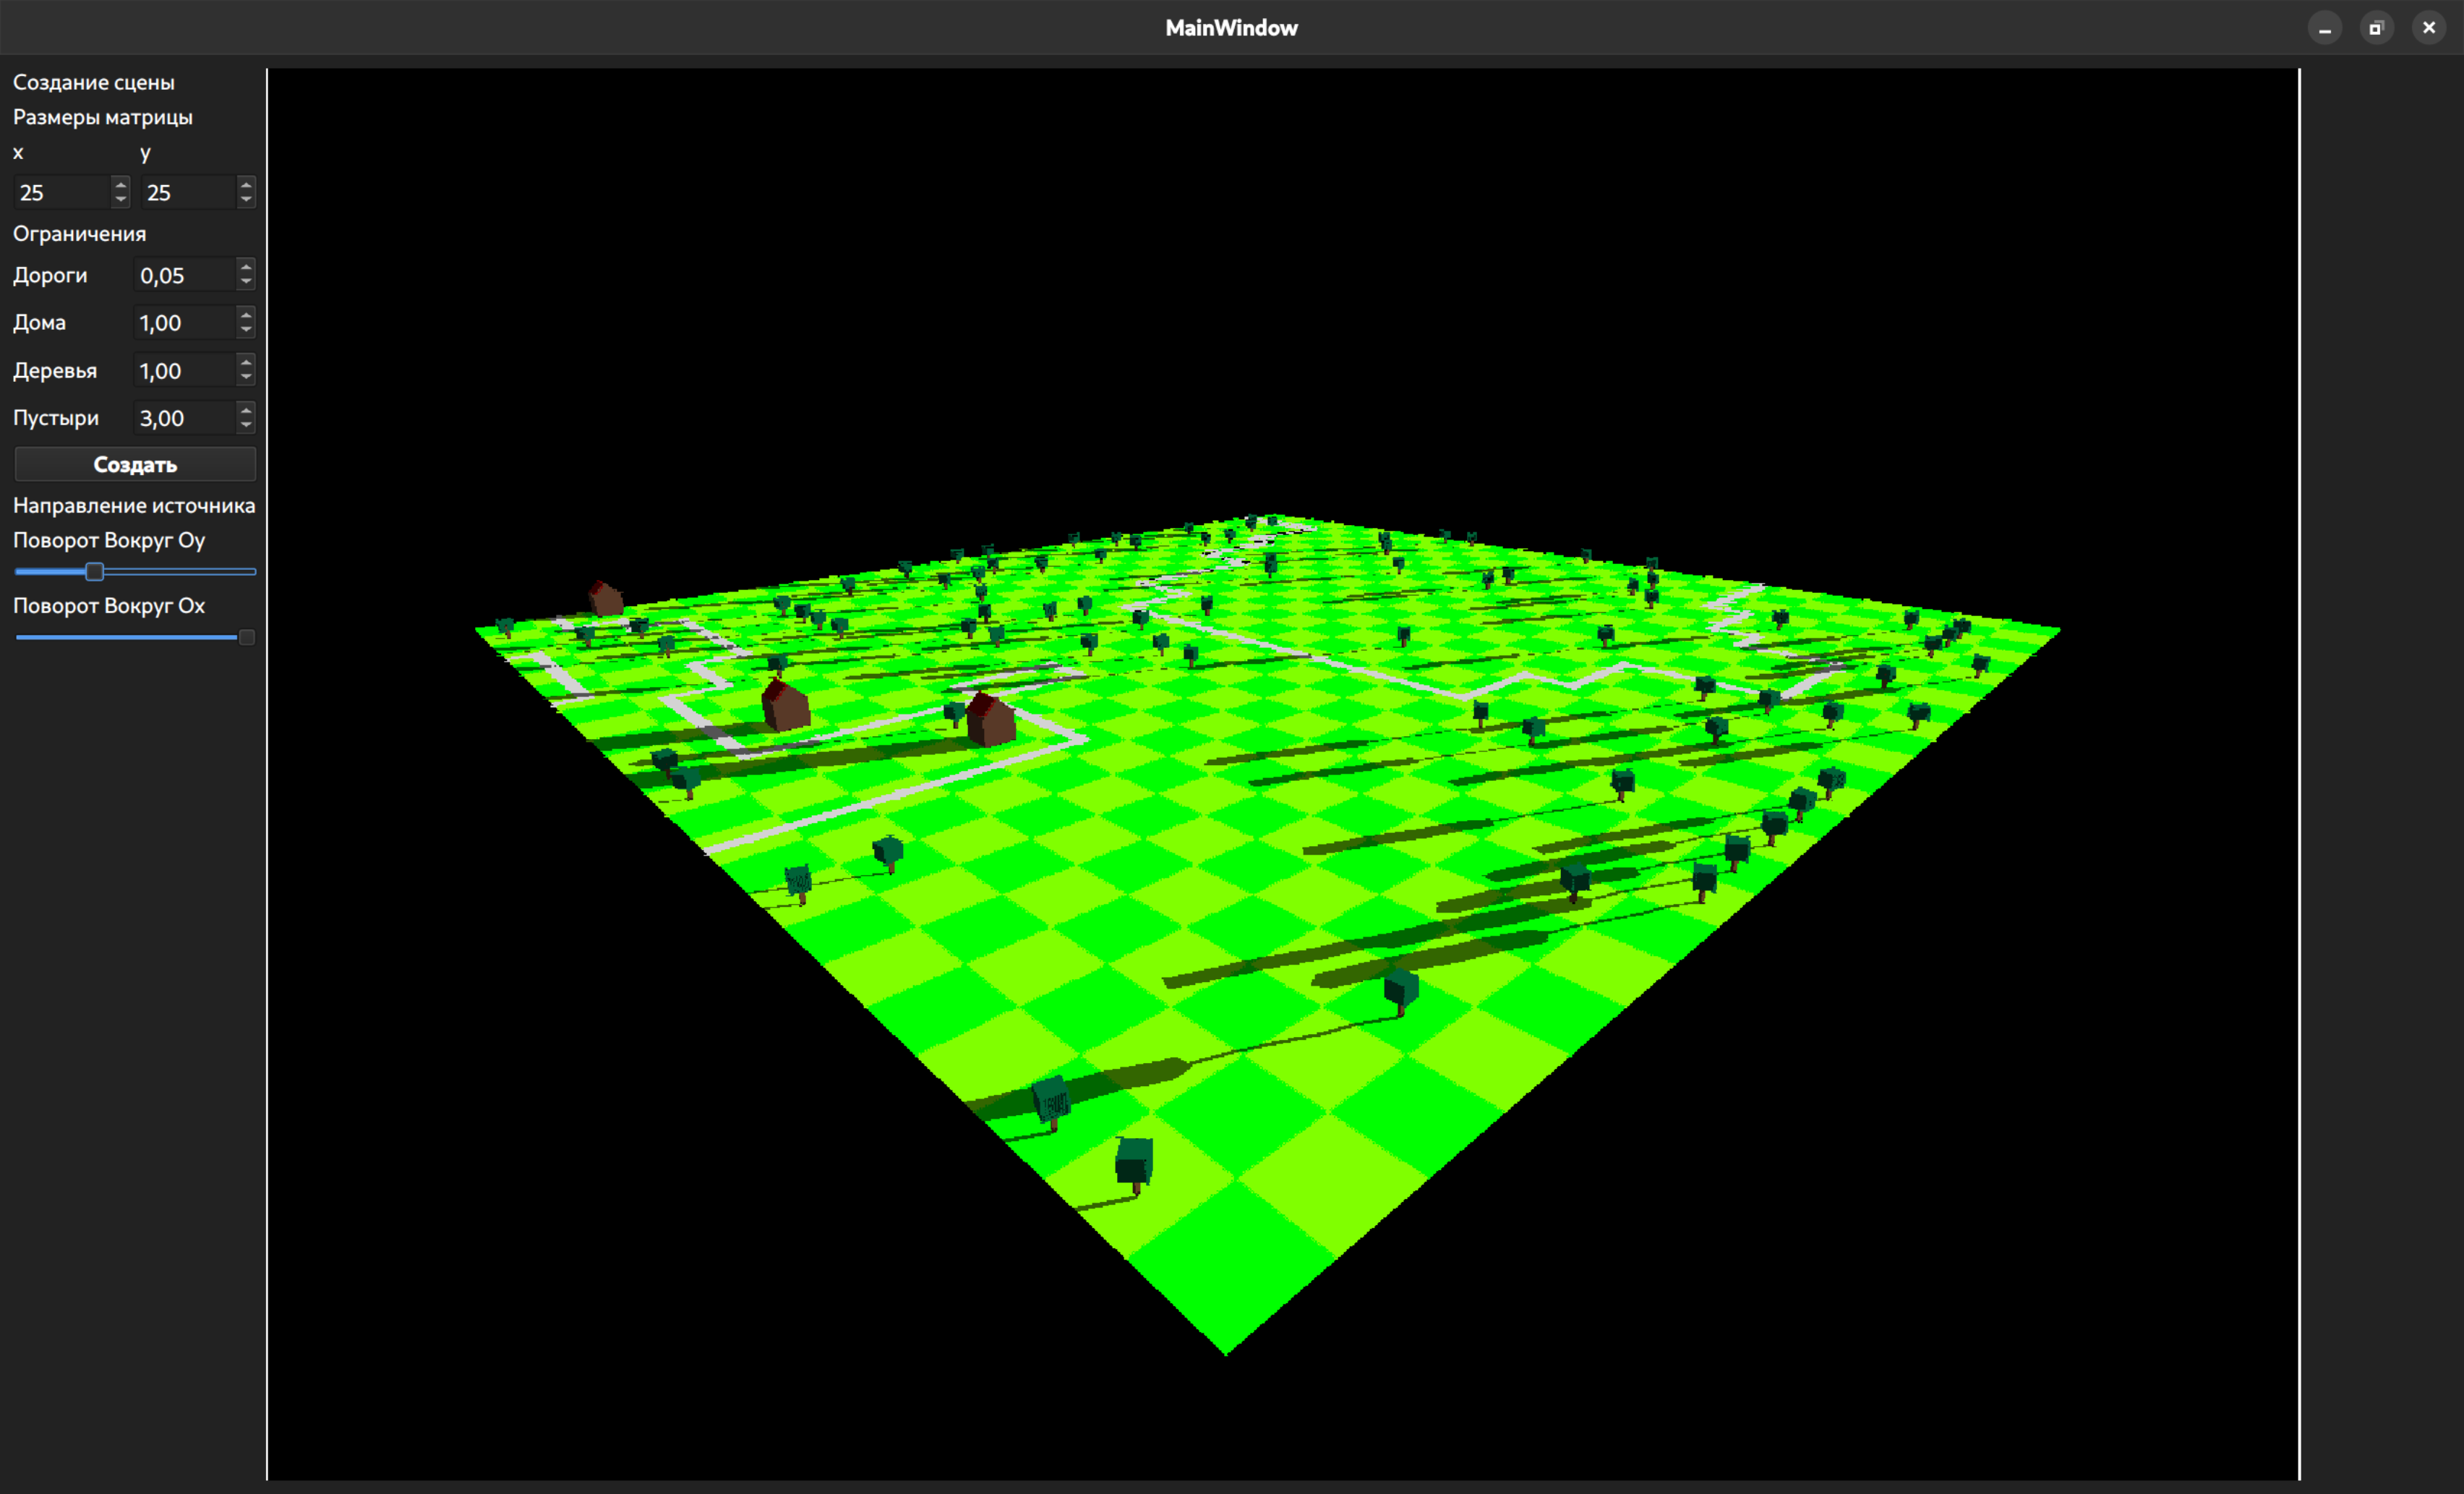
\includegraphics[width=\textwidth]{pic4}
  \caption{Пример работы программы --- Источник света приближен к земле, тени становятся длиннее}
  \label{fig:example_4}
\end{figure}
\begin{figure}[h!]
  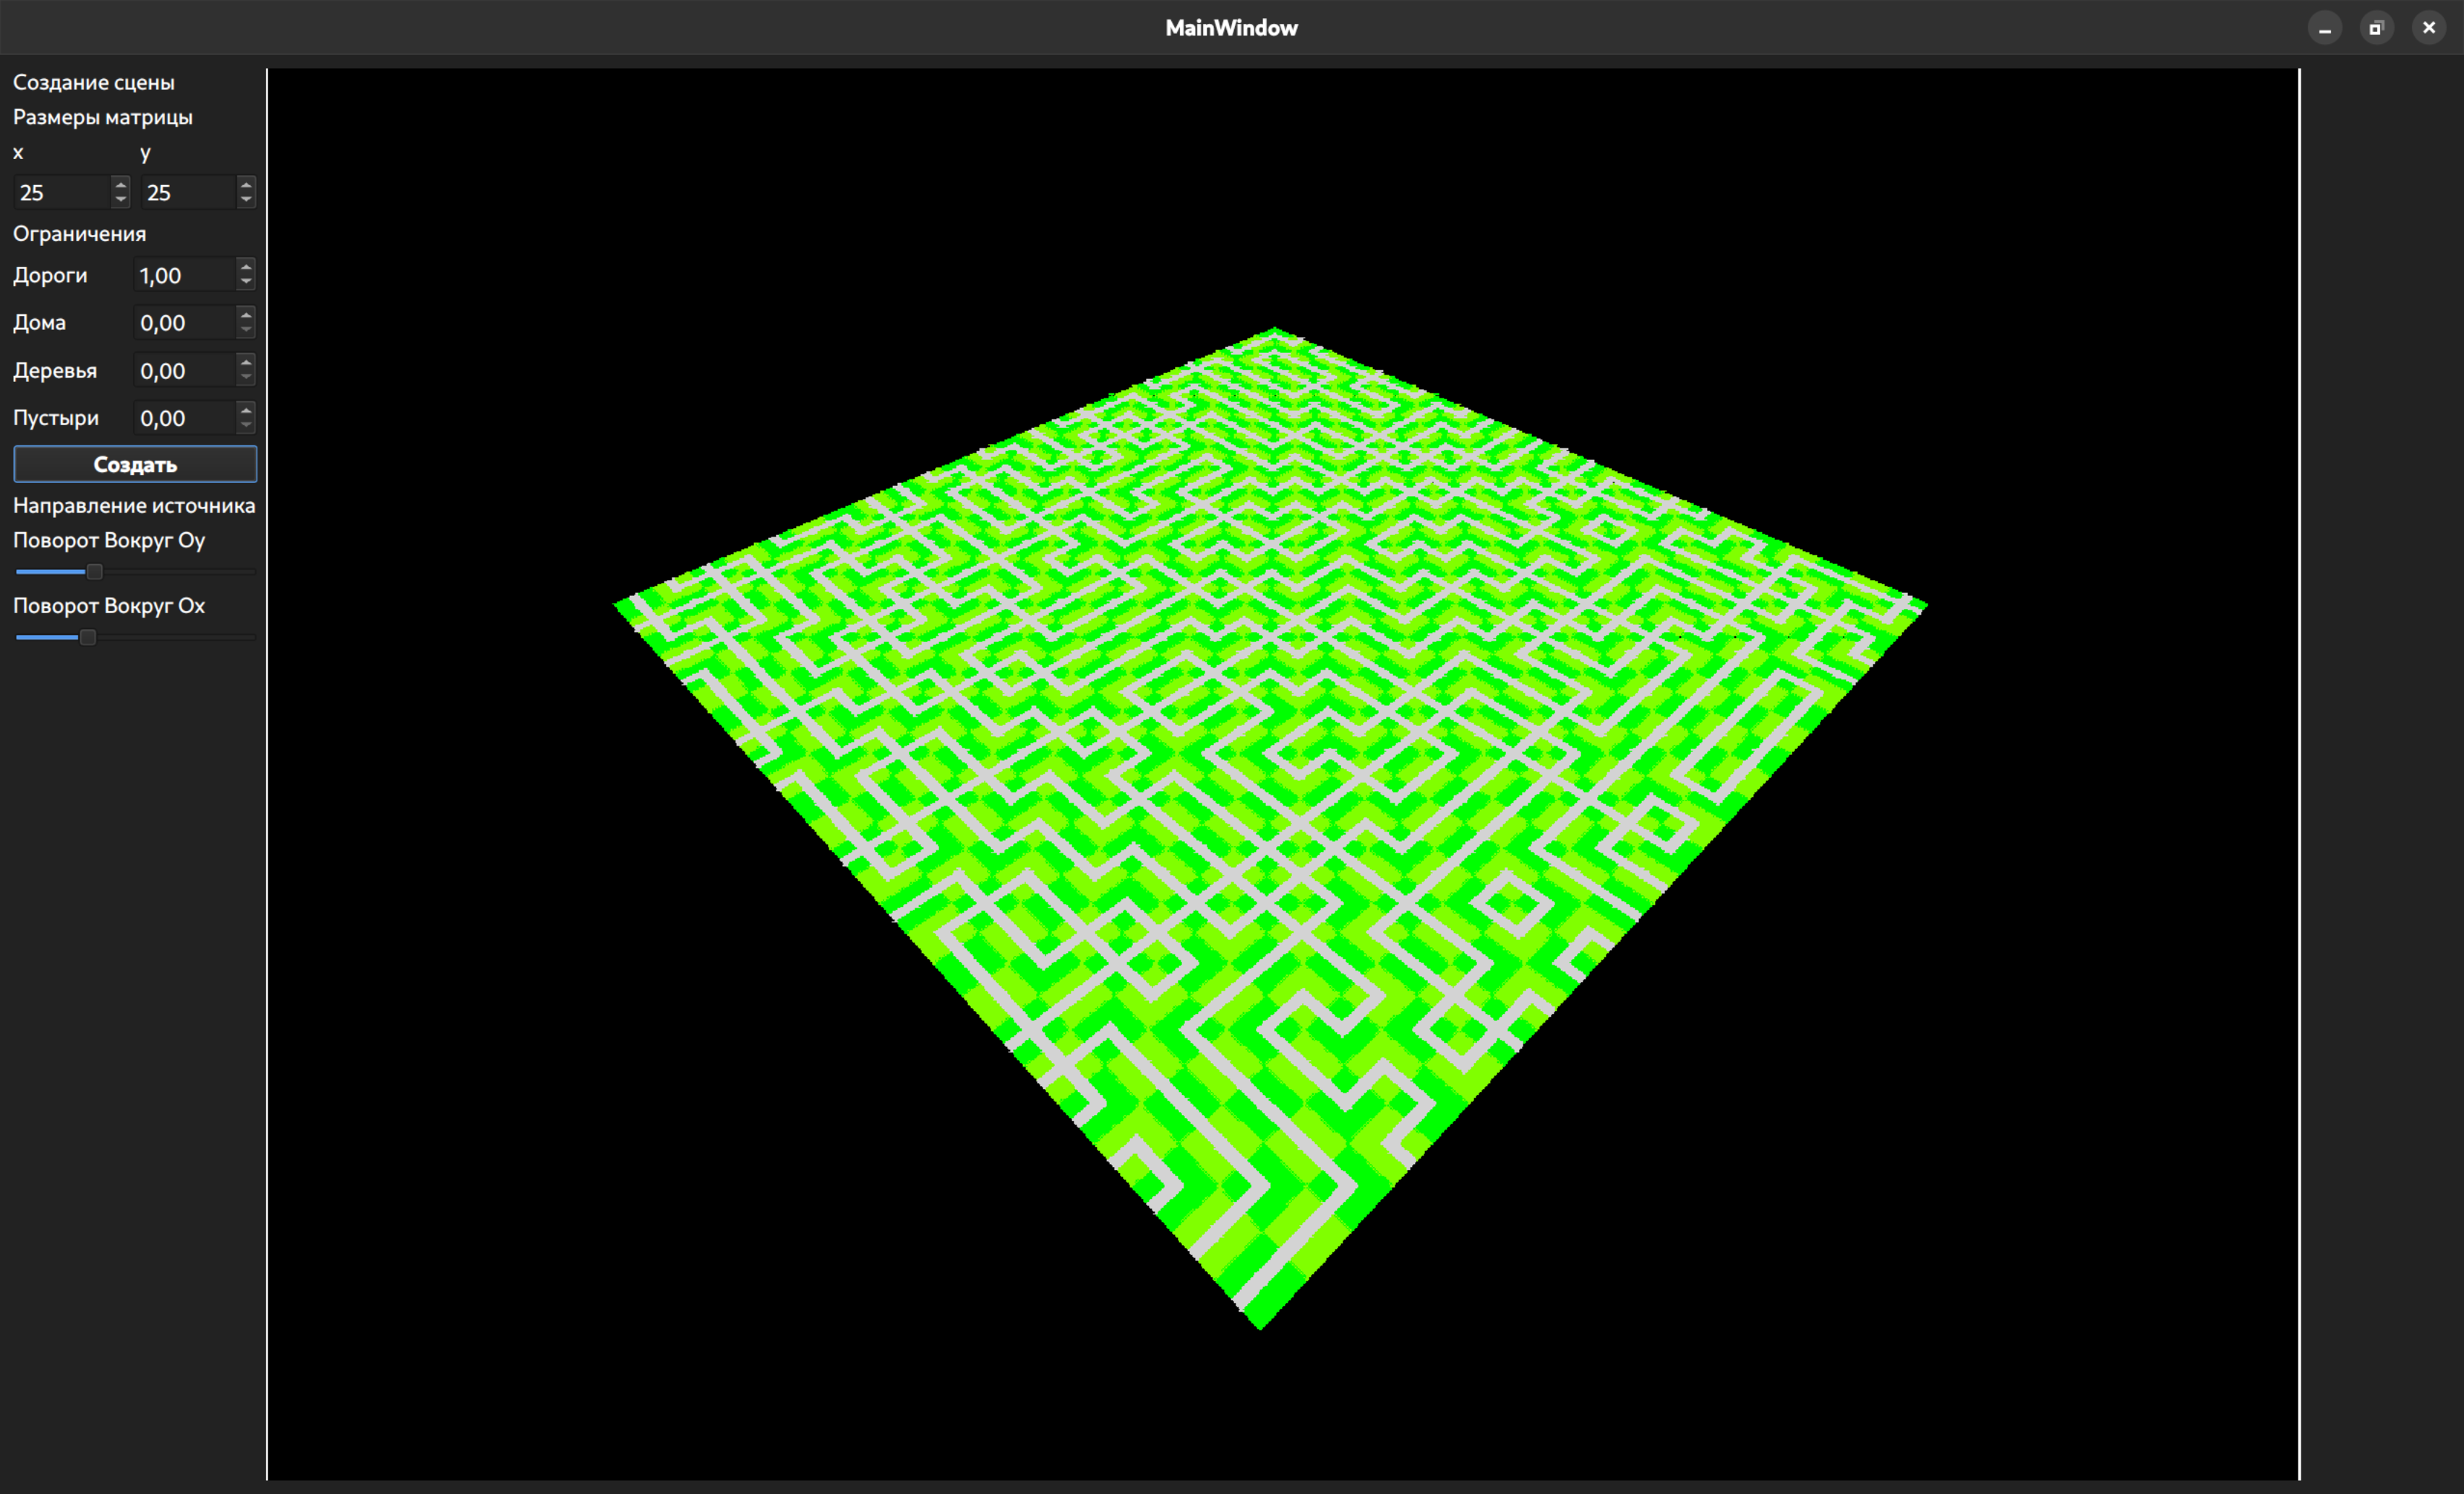
\includegraphics[width=\textwidth]{pic5}
  \caption{Пример работы программы --- запрещено появление любых объектов кроме дорог}
  \label{fig:example_5}
\end{figure}

\newpage

\

\section{Вывод}

Была осуществлена реализация программного обеспечения для создания конструирования и визуализации загородного посёлка.